\subsection{Diagrama de Actividades}
\label{subsec:diagramas_actividades_quejoso}

El comportamiento dinámico y la experiencia de navegación del quejoso se modelan mediante un diagrama de actividades que describe los flujos que el quejoso puede llevar a través de la plataforma. Para facilitar la visibilidad del diagrama se divide en 2 figuras siguientes.
Esta primera figura representa el punto de entrada al sistema desde el Portal de inicio de la Defensoría. Describe las opciones disponibles para el usuario antes de contar con una sesión activa, tales como el seguimiento rápido de expedientes existentes y el proceso principal de presentar una queja. En este último, se modela la lógica de validación para menores de edad y la captura narrativa de los hechos hasta la generación del folio de éxito. El flujo concluye en un punto de decisión donde el usuario, tras recibir su acuse, determina si desea "Continuar como invitado" o proceder a la "Configuración de Cuenta” para formalizar su acceso al sistema

\begin{figure}[H]
    \centering
    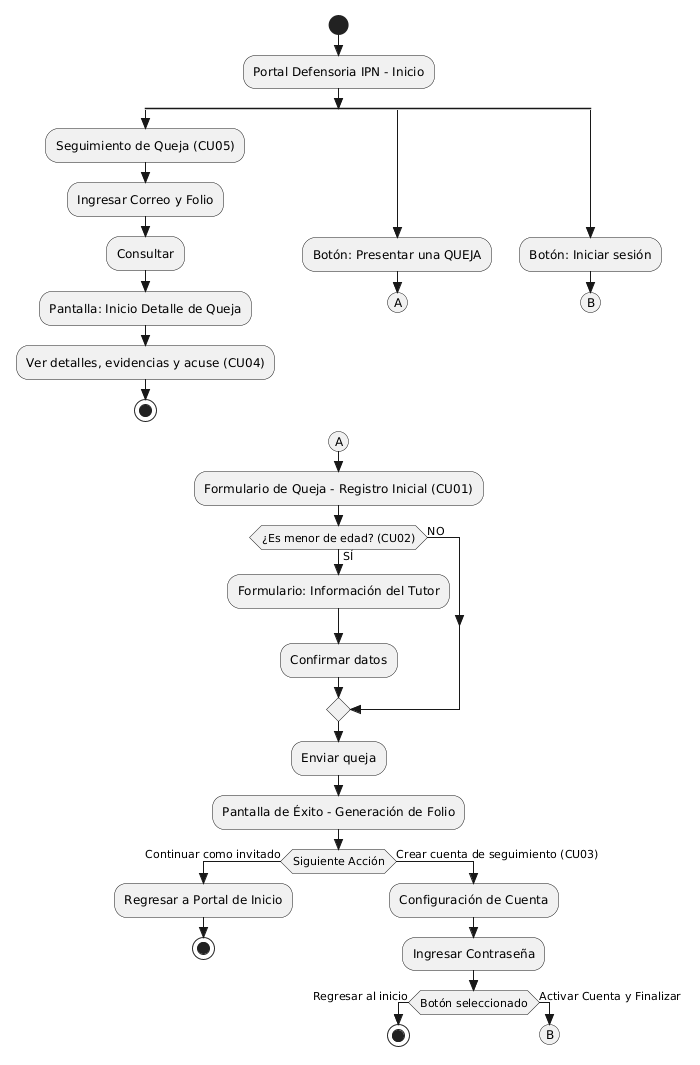
\includegraphics[width=\textwidth, height=0.85\textheight, keepaspectratio]{imagenes/quejoso/D_Actividad/P1_DA-Quejoso.png}
    \caption{Diagrama de Actividades: Flujo de Navegación del Quejoso (Parte 1)}
    \label{fig:da_quejoso_p1}
\end{figure}

La segunda figura comienza con el nodo de "Iniciar Sesión”, el cual puede ser alcanzado desde el portal de inicio, tras la creación de una cuenta o desde el flujo de activación por folio. Se integran las vías alternativas de soporte, como el restablecimiento de credenciales ante el olvido de contraseñas. Una vez superada la autenticación, se describe la navegación cíclica dentro del Dashboard, donde el quejoso interactúa con su resumen de expedientes, historial, levantamiento de nuevas denuncias y el centro de notificaciones para la toma de decisiones sobre propuestas de conciliación. El flujo permanece activo en este entorno de gestión hasta que el usuario ejecuta la acción de cierre de sesión o haya expirado esta.

\begin{figure}[H]
    \centering
    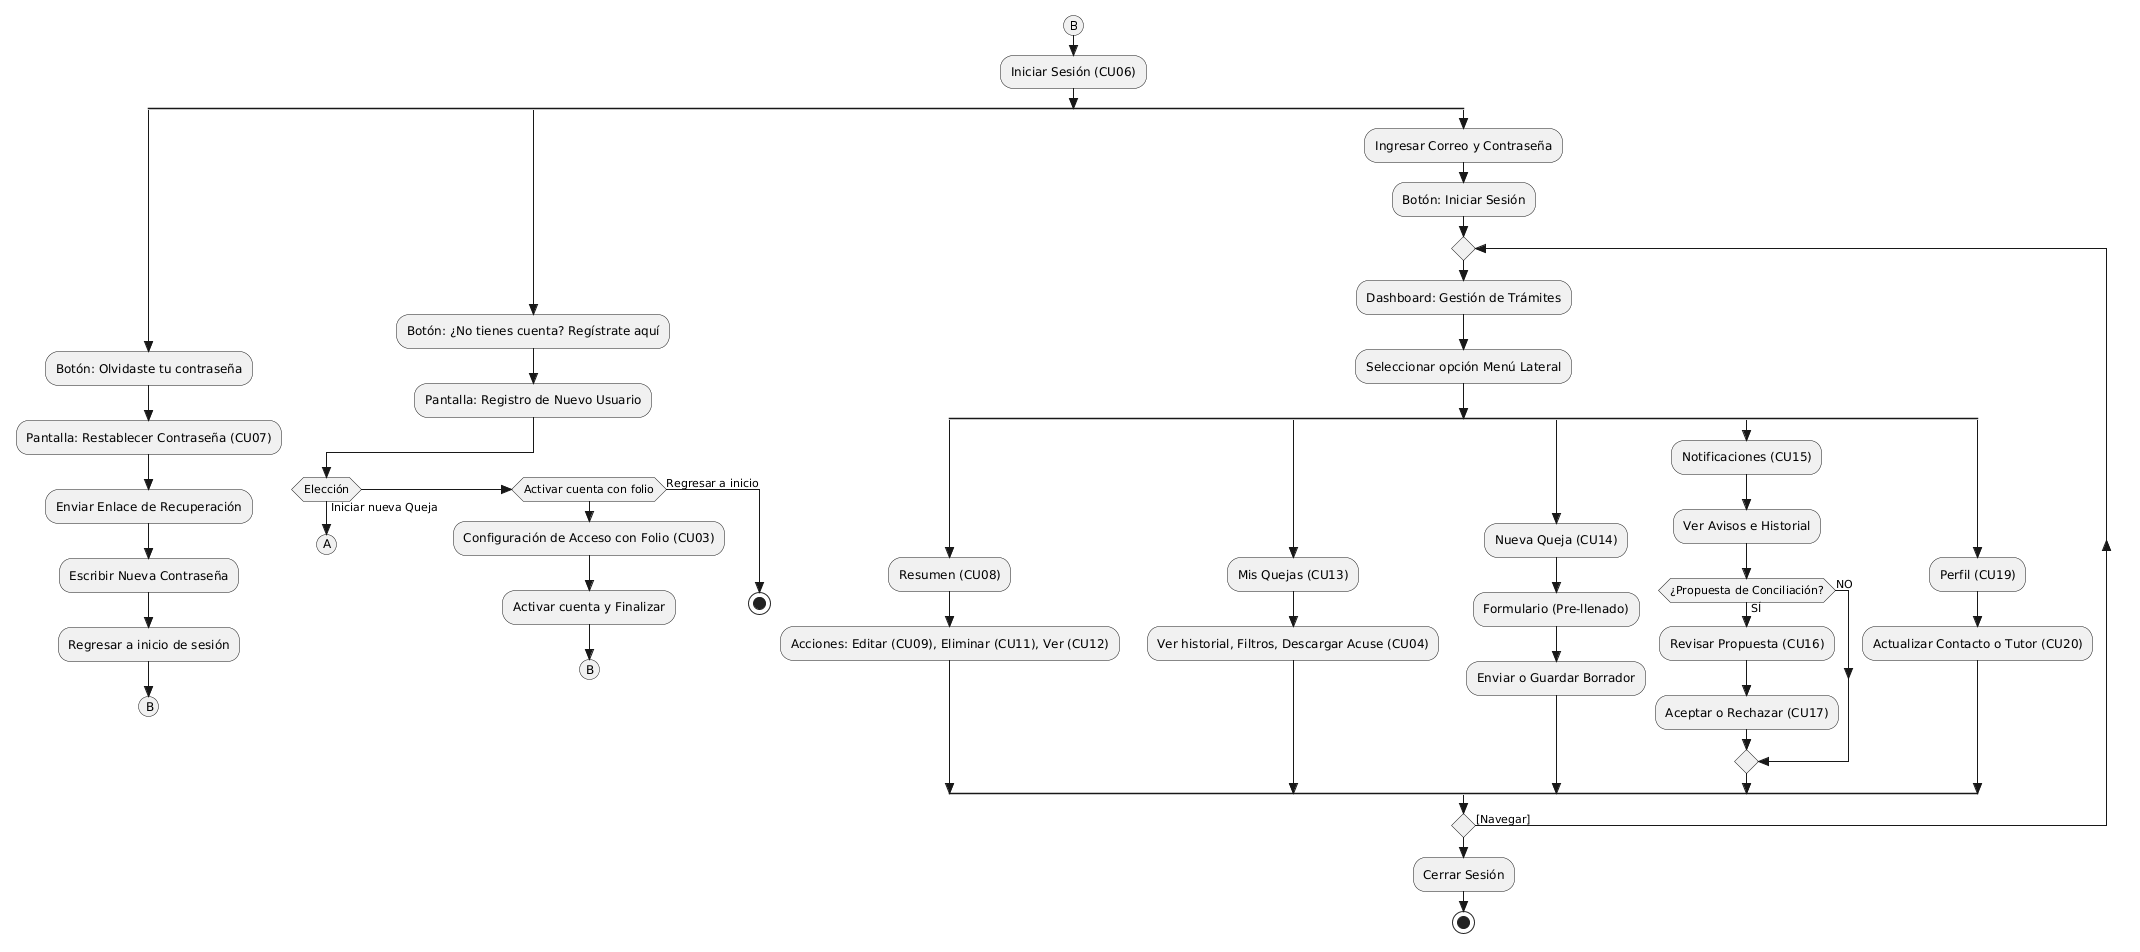
\includegraphics[width=\textwidth]{imagenes/quejoso/D_Actividad/P2_DA-Quejoso.png}
    \caption{Diagrama de Actividades: Flujo de Navegación del Quejoso (Parte 2)}
    \label{fig:da_quejoso_p2}
\end{figure}
